\documentclass[tikz,border=10pt]{standalone}

\begin{document}
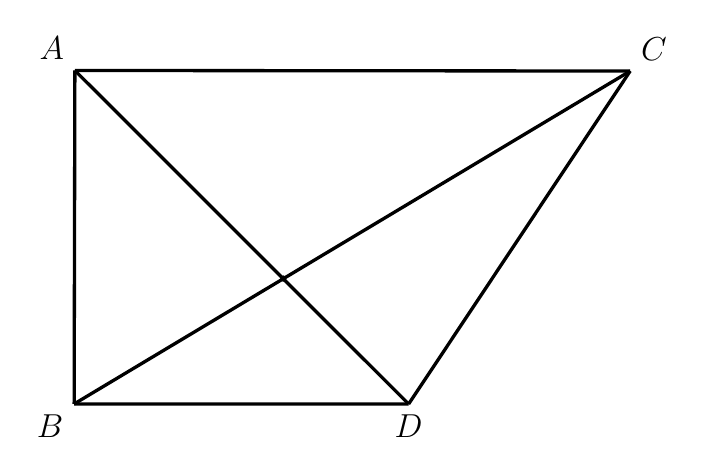
\begin{tikzpicture}[line join=round, line width=1.2pt]
\coordinate (A) at (-3.531,2.278);
\coordinate (B) at (-3.540,-1.957);
\coordinate (C) at (3.522,2.271);
\coordinate (D) at (0.708,-1.958);

  
  \draw (A) -- (C);   
  \draw (A) -- (B);   
  \draw (B) -- (D);   
  \draw (A) -- (D);   
  \draw (B) -- (C);   
  \draw (D) -- (C);   

  
  \fill (-0.883,-0.365) circle (0.040);

  
  \node[above left, font=\fontsize{12}{14.4}\selectfont] at (A) {$A$};
  \node[below left, font=\fontsize{12}{14.4}\selectfont] at (B) {$B$};
  \node[above right, font=\fontsize{12}{14.4}\selectfont] at (C) {$C$};
  \node[below, font=\fontsize{12}{14.4}\selectfont] at (D) {$D$};
\end{tikzpicture}
\end{document}